\documentclass[openany]{tietreport}

% Import images
\usepackage{graphicx}

% Bibliography configuration
\usepackage[
  date=year,
  style=alphabetic,
  backend=biber,
  sorting=nty,
  maxnames=5,
  minnames=3,
  maxalphanames=4,
  minalphanames=3,
  backref=true,
  doi=false,
  isbn=false,
  url=true,
  eprint=false
]{biblatex}
\begin{filecontents*}{donna_sources.bib}
@online{electron,author={{Electron}},title={Electron Documentation},url={https://www.electronjs.org/docs/latest/}}
@online{capture,author={{Electron}},title={desktopCapturer API},url={https://www.electronjs.org/docs/latest/api/desktop-capturer}}
@online{ipc,author={{Electron}},title={Inter-Process Communication},url={https://www.electronjs.org/docs/latest/tutorial/ipc}}
@online{worklet,author={{MDN Web Docs}},title={AudioWorklet},url={https://developer.mozilla.org/en-US/docs/Web/API/AudioWorklet}}
@online{media,author={{MDN Web Docs}},title={MediaDevices},url={https://developer.mozilla.org/en-US/docs/Web/API/MediaDevices}}
@article{whisper,author={Radford, Alec and Kim, Jong Wook and Xu, Tao and Brockman, Greg and McLeavey, Christine and Sutskever, Ilya},title={Robust Speech Recognition via Large-Scale Weak Supervision},journal={Proceedings of ICML},year={2023}}
@online{gemini,author={{Google}},title={Gemini API Documentation},url={https://ai.google.dev/gemini-api/docs}}
\end{filecontents*}
\addbibresource{donna_sources.bib}

%% ==================================================
%% CUSTOMIZE THESE FIELDS FOR YOUR PROJECT
%% ==================================================

% Course/Lab header
\TitlePageHeader{%
  UCS 503 Software Engineering Project Report%
}

% Main project title
\ProjectTitle{%
  Donna: Real-Time Desktop AI Copilot%
}

% Subtitle or project description
\ProjectSubTitle{%
  Multimodal Screen and Audio Context for Desktop Assistance%
}

% Student information (up to 4 students)
\author{%
  \texttt{1024170400} Samyak Jain \\
  \texttt{1024170388} Sangam Sangwan%
}

% Group number, degree, year, program
\TitlePageSubText{%
  BE Third Year, CSE%
}

% Faculty advisor/guide name
\AdvisorName{%
  Ms Paramveer Sidhu%
}

% Evaluation period and department info
\TitlePageFooterText{{%
    \large End-Semester Evaluation \\[0.2cm]
    \bfseries Computer Science and Engineering
    Department%
  } \\[0.15cm]
  Thapar Institute of Engineering and Technology,
  Patiala%
}

%% ==================================================


\usepackage{tikz,booktabs,tabularx,float}
\usetikzlibrary{arrows.meta,positioning,fit,shapes.geometric}
\makeatletter
\@openrightfalse
\makeatother
\setlength{\headheight}{15pt}
\raggedbottom
\setlength{\textfloatsep}{10pt}
\setlength{\intextsep}{10pt}
\tikzset{stage/.style={draw=blue!55!black,fill=blue!5,rounded corners=2pt,align=center,font=\small,minimum height=9mm,text width=32mm},link/.style={-{Stealth},thick,draw=blue!55!black}}


\begin{document}
\maketitle
\tableofcontents
\chapter{Introduction}
\section{Background and Context}
Donna is a desktop AI copilot that combines screen content and live conversation context in a floating interface. It allows a user to ask about visible material, obtain assistance with an ongoing discussion, request follow-up questions and generate a recap without manually transferring information into a separate chat application.
\subsection{Problem Statement}
Screen content and spoken discussion are normally available through separate applications. A useful desktop assistant must acquire both, preserve the distinction between local and remote speech, and assemble the relevant information into a model request. The engineering challenge is to coordinate capture, transcription and inference without blocking the interface or leaving capture resources active after a session ends.
\section{Project Objectives}
The completed scope comprises desktop overlay interaction, screenshot-based assistance, independent microphone and system audio acquisition, speech segmentation and transcription, conversation context assembly, and on-demand AI answers, follow-ups and recaps. The final milestone extends the screen-only midterm implementation with the complete audio-to-answer pipeline.
\begin{table}[htbp]\centering\small
\begin{tabularx}{\linewidth}{@{}lXX@{}}\toprule
Capability & Midterm & Final milestone \\ \midrule
Desktop interface & Floating assistant & Integrated screen and audio controls \\
Visual context & Screenshot questions & Available alongside conversation context \\
Audio & Planned & Microphone and system playback \\
Speech recognition & Planned & Local Whisper and configurable STT \\
Assistance & Screen questions & Answers, follow-ups and recaps \\
\bottomrule\end{tabularx}\caption{Progression from midterm to final scope}\end{table}
\chapter{Methodology and Design}
\section{System Architecture}
\subsection{High-Level Design}
Donna separates acquisition, context management and inference. Screen capture supplies a snapshot, while audio capture produces a sequence of source-labelled utterances. These paths converge only when an assistance request is assembled. This separation allows transcription to continue independently of AI response generation.
\begin{figure}[htbp]\centering
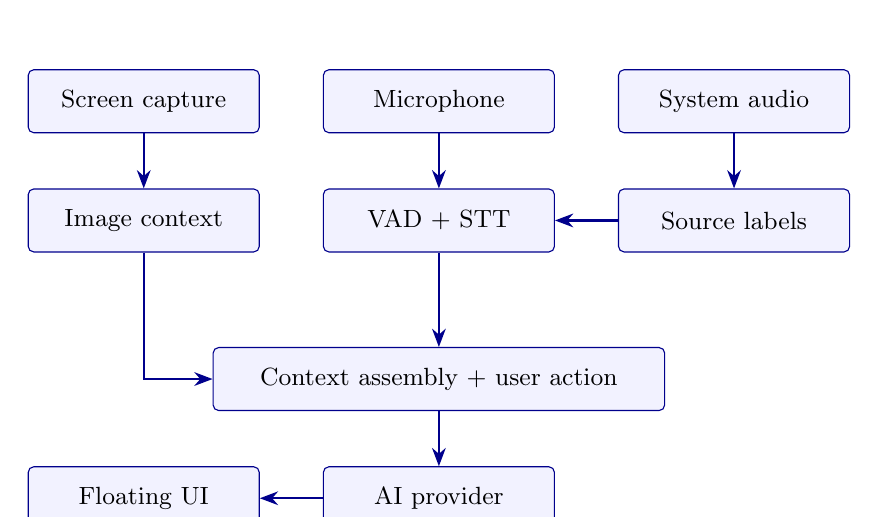
\begin{tikzpicture}[node distance=7mm and 8mm,stage/.append style={text width=27mm,minimum height=8mm}]
\node[stage](screen){Screen capture};\node[stage,right=of screen](mic){Microphone};\node[stage,right=of mic](sys){System audio};
\node[stage,below=of screen](image){Image context};\node[stage,below=of mic](stt){VAD + STT};\node[stage,below=of sys](labels){Source labels};
\node[stage,below=12mm of stt,text width=55mm](ctx){Context assembly + user action};\node[stage,below=of ctx](ai){AI provider};\node[stage,left=of ai](ui){Floating UI};
\draw[link](screen)--(image);\draw[link](mic)--(stt);\draw[link](sys)--(labels);\draw[link](labels)--(stt);\draw[link](image)|-(ctx);\draw[link](stt)--(ctx);\draw[link](ctx)--(ai);\draw[link](ai)--(ui);
\end{tikzpicture}\caption{Logical multimodal architecture}\end{figure}
\subsection{Technical Stack}
\begin{table}[htbp]\centering\small\begin{tabularx}{\linewidth}{@{}lX@{}}\toprule
Technology & Role in Donna \\ \midrule
Electron, Node.js & Desktop runtime, window lifecycle and privileged operations \\
HTML, CSS, JavaScript & Floating interface and interaction state \\
Electron IPC & Communication across renderer and main process \\
Web Audio, AudioWorklet & Audio frame acquisition \\
Local Whisper & Batch speech recognition \\
Gemini & Demonstrated multimodal answer generation \\
\bottomrule\end{tabularx}\caption{Implementation stack}\end{table}
\section{Implementation Details}
\subsection{Desktop interface and process boundaries}
The floating interface is the entry point for screen questions and conversation assistance. Electron separates the renderer from privileged desktop operations through a preload and IPC boundary \cite{electron,ipc}. The renderer handles user actions, audio acquisition and presentation; the main process coordinates desktop services and provider-facing operations. Requests and returned results cross this boundary asynchronously, so the interface must distinguish a pending operation from a completed one.
\begin{figure}[htbp]\centering
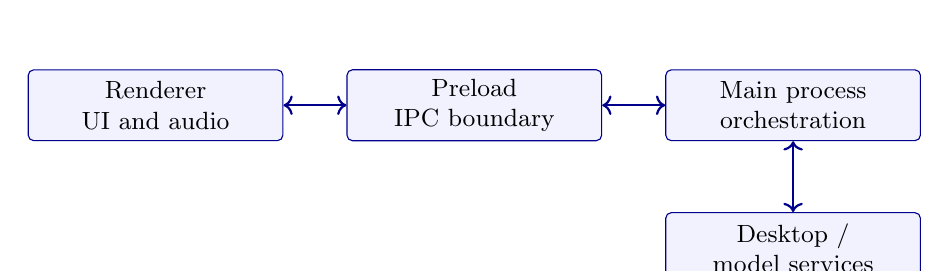
\begin{tikzpicture}[node distance=9mm and 8mm,stage/.append style={text width=30mm}]
\node[stage](ui){Renderer\\UI and audio};\node[stage,right=of ui](ipc){Preload\\IPC boundary};\node[stage,right=of ipc](main){Main process\\orchestration};
\node[stage,below=of main](services){Desktop / model services};\draw[link,<->](ui)--(ipc);\draw[link,<->](ipc)--(main);\draw[link,<->](main)--(services);
\end{tikzpicture}\caption{Electron component boundaries (logical view)}\end{figure}
\subsection{Screen capture and visual assistance}
The screen workflow uses Electron desktop capture \cite{capture}. A screenshot is associated with the user's question and submitted to a model capable of interpreting images. The returned answer is rendered in the floating interface. Unlike a text-only workflow, the image preserves visual layout, code formatting and other spatial information. Capture is performed for relevant requests rather than treating every desktop frame as a model input.
\subsection{Dual-source audio acquisition}
Microphone input represents the local speaker (You); system loopback represents playback from the computer (Them). Maintaining these as separate streams avoids the need to infer speaker identity from a mixed recording. The labels identify input sources, not individual speakers in a multi-person call.

AudioWorklet processing obtains audio frames from each stream \cite{worklet,media}. The speech pipeline prepares the frames for recognition through format conversion, buffering and voice activity detection. The source association must survive each processing stage so that the final transcript can be attributed correctly.
\begin{figure}[htbp]\centering
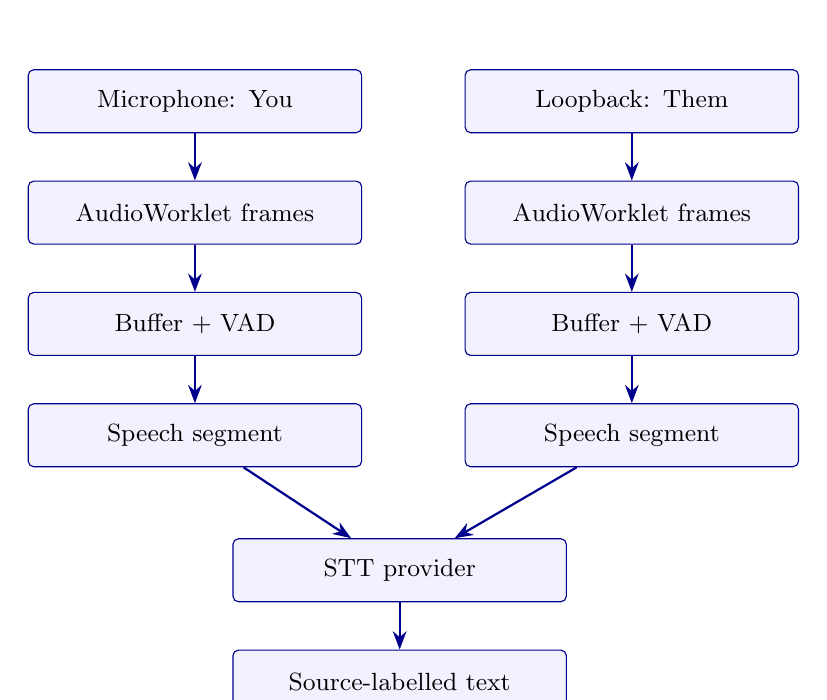
\begin{tikzpicture}[node distance=6mm and 13mm,stage/.append style={text width=40mm,minimum height=8mm}]
\node[stage](m){Microphone: You};\node[stage,right=of m](s){Loopback: Them};
\node[stage,below=of m](mw){AudioWorklet frames};\node[stage,below=of s](sw){AudioWorklet frames};
\node[stage,below=of mw](mb){Buffer + VAD};\node[stage,below=of sw](sb){Buffer + VAD};
\node[stage,below=of mb](mt){Speech segment};\node[stage,below=of sb](st){Speech segment};
\node[stage,below=9mm of mt,xshift=26mm](w){STT provider};\node[stage,below=of w](out){Source-labelled text};
\foreach \a/\b in {m/mw,s/sw,mw/mb,sw/sb,mb/mt,sb/st,mt/w,st/w,w/out}{\draw[link](\a)--(\b);}
\end{tikzpicture}\caption{Independent audio paths and logical source preservation}\end{figure}
\subsection{Speech segmentation and transcription}
Voice activity detection identifies speech regions and supports utterance finalization. Rather than issuing a recognition request for every incoming frame, the local path accumulates frames into speech segments and submits finalized buffers for batch transcription. This reduces unnecessary recognition calls, at the cost of waiting for a segment boundary. Whisper provides the local recognition path \cite{whisper}.

The application exposes Auto, Local, Deepgram, OpenAI and Gemini STT selections. Local Whisper was used in the demonstrated workflow; cloud choices depend on credentials and provider availability. Recognition produces text independently of the answer action, allowing the user to review the conversation before requesting inference.
\subsection{Conversation context and AI inference}
The context layer combines the user request, relevant screenshot and recent source-labelled transcript. A rolling context design limits unnecessary prompt growth. The distinction between You and Them provides conversational structure without claiming individual speaker diarization.

Donna supports three conversation actions: Answer uses the current discussion to generate assistance; Follow-up requests additional questions or clarification; Recap summarizes the discussion. Screen questions can use the captured image as visual evidence. Gemini was used for the demonstrated integrated response \cite{gemini}. STT and AI inference are separate provider responsibilities, so a model error need not imply a capture failure.
\begin{figure}[htbp]\centering
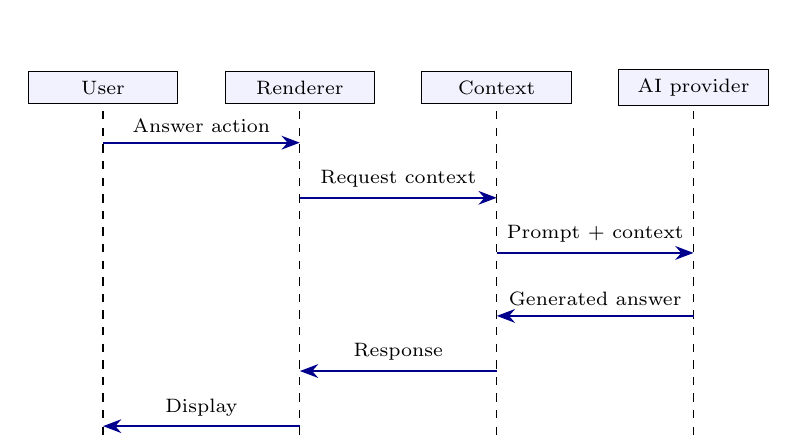
\begin{tikzpicture}[x=1cm,y=1cm,font=\scriptsize]
\foreach \x/\n in {0/User,2.5/Renderer,5/Context,7.5/AI provider}{\node[draw,fill=blue!5,minimum width=19mm] at (\x,0){\n};\draw[dashed](\x,-.3)--(\x,-4.6);}
\draw[link](0,-.7)--node[above]{Answer action}(2.5,-.7);
\draw[link](2.5,-1.4)--node[above]{Request context}(5,-1.4);
\draw[link](5,-2.1)--node[above]{Prompt + context}(7.5,-2.1);
\draw[link](7.5,-2.9)--node[above]{Generated answer}(5,-2.9);
\draw[link](5,-3.6)--node[above]{Response}(2.5,-3.6);
\draw[link](2.5,-4.3)--node[above]{Display}(0,-4.3);
\end{tikzpicture}\caption{Logical sequence of an on-demand answer request}\end{figure}
\subsection{Session lifecycle and failure handling}
Capture sessions have distinct initialization, acquisition and cleanup phases. Repeated starts must not create duplicate active processors. Stopping a session requires releasing media tracks and worklet resources and preventing stale callbacks from affecting the next session. During development, duplicate starts and repeated invocation of a one-time callback were identified as failure modes. The integrated restart workflow was subsequently reported working.
\begin{figure}[htbp]\centering
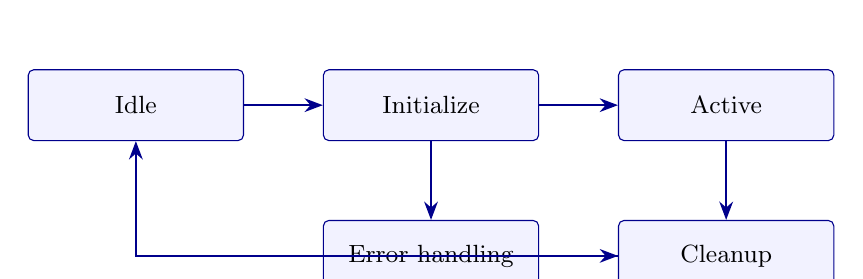
\begin{tikzpicture}[node distance=10mm and 10mm,stage/.append style={text width=25mm}]
\node[stage](idle){Idle};\node[stage,right=of idle](init){Initialize};\node[stage,right=of init](active){Active};\node[stage,below=of active](stop){Cleanup};\node[stage,below=of init](err){Error handling};
\draw[link](idle)--(init);\draw[link](init)--(active);\draw[link](active)--(stop);\draw[link](stop)-|(idle);\draw[link](init)--(err);\draw[link](err)--(stop);
\end{tikzpicture}\caption{Logical capture lifecycle and recovery paths}\end{figure}
\subsection{Design decisions}
\begin{table}[htbp]\centering\small\begin{tabularx}{\linewidth}{@{}lX@{}}\toprule Decision & Engineering rationale \\ \midrule
Separate audio streams & Preserve source context without mixed-stream diarization. \\
Batch local STT & Avoid per-request cloud STT fees; accept segment-finalization delay. \\
Explicit inference actions & Avoid generating an answer for every utterance. \\
Separate provider stages & Isolate recognition failures from model inference failures. \\
Session cleanup & Enable repeatable capture without duplicate processors. \\
\bottomrule\end{tabularx}\caption{Key design trade-offs}\end{table}
Local STT reduces raw-audio transmission to external recognition services, but transcripts and images may still be sent to the selected AI provider. Audio capture requires appropriate consent.
\chapter{Results and Evaluation}
\section{Testing Methodology}
The team evaluated the application on its laptops. Midterm trials established the screenshot workflow. Final development observations cover microphone and loopback capture, speech segmentation, local Whisper transcription, transcript publication, Gemini answer generation and session restart. The evaluation follows the pipeline stage by stage to distinguish capture, recognition and inference failures.
\begin{table}[htbp]\centering\small\begin{tabularx}{\linewidth}{@{}lXX@{}}\toprule
Test & Expected outcome & Observed evidence \\ \midrule
Desktop UI & Open and interact & Local laptop trials \\
Screen question & Image-aware response & Midterm functional tests \\
Microphone & Local speech input & Capture logs \\
System audio & Playback input & Loopback logs \\
Local STT & Segment becomes text & Whisper workflow demonstrated \\
AI answer & Context-based response & Gemini response reported \\
Restart & New session after stop & Restart reported \\
Follow-up / recap & Requested assistance & Completed scope; separate test records unavailable \\
\bottomrule\end{tabularx}\caption{Functional requirements and evaluation evidence}\end{table}
\section{Performance Metrics}
The evaluation establishes functional operation rather than numerical performance. Controlled measurements of transcription latency, word error rate and AI response time were not supplied; no numerical claims are made. For future repeatable measurements, recognition latency should be timed from segment finalization to transcript publication, separately from model response latency.
\section{Analysis}
The principal integration result is the progression from a screen-aware assistant to an audio-aware assistant with independent capture, transcription and inference stages. Development debugging showed why a successful capture-start message alone is insufficient: a complete test must also observe segment finalization, transcript publication and the requested AI response.
\begin{table}[htbp]\centering\small\begin{tabularx}{\linewidth}{@{}lX@{}}\toprule
Issue & Diagnostic approach \\ \midrule
Duplicate capture starts & Trace session initialization and cleanup boundaries. \\
Repeated one-time callback & Inspect asynchronous completion and callback ownership. \\
Transcript not visible & Trace VAD, recognition and publication separately. \\
Provider model failure & Check inference independently of successful transcription. \\
\bottomrule\end{tabularx}\caption{Integration challenges and debugging approach}\end{table}
The strongest evidence is the integrated local audio-to-answer workflow and the earlier screen workflow. Noise, hardware resources and provider availability remain practical constraints.
\chapter{Conclusion}
\section{Summary of Work}
Donna delivers the planned desktop copilot scope: floating interaction, screenshot assistance, independent microphone and system audio capture, speech segmentation, local transcription, conversation context and on-demand AI assistance. The final milestone integrates the visual and audio paths into a single application.
\section{Key Findings}
Separating audio sources preserves useful conversational structure. Separating transcription from inference gives the user control over model requests and makes debugging more precise. Session lifecycle management is essential to repeatable operation.
\section{Future Work and Recommendations}
Future improvements concern measured latency and recognition accuracy, noise robustness, broader platform testing and automated regression coverage rather than unfinished core features.
\section{Final Remarks}
The project demonstrates practical desktop software engineering through the integration of asynchronous media acquisition, local speech recognition and multimodal model inference.
\printbibliography[heading=bibintoc]
\end{document}
